\documentclass[11pt]{article}
\usepackage[margin=1in]{geometry}
\usepackage{booktabs}
\usepackage{graphicx}
\usepackage{amsmath}
\begin{document}
\title{Ballistic-Coefficient Sweep Test for the Cape Cod Bay Bolide}
\author{Generated analysis note}
\maketitle
\section*{Purpose}
This test is separate from the manuscript draft.  For each fixed value of the drag-area-to-mass parameter $C_D A/m$, the six GCRS initial-state components are refit while $C_D A/m$ is held fixed.  Increasing $C_D A/m$ corresponds to decreasing the conventional ballistic coefficient $m/(C_D A)$ and therefore to a smaller dynamically allowed mass for a fixed spherical density.  The manuscript fit product is only read; it is not overwritten.

\section*{Setup}
The baseline fit product is \texttt{\detokenize{products/ballistic_head_trail_correlated_appendix_fit/ballistic_head_trail_correlated_fit.json}}.  The baseline version is \texttt{0.2.1}.  The nominal $C_D A/m$ is 4.021e-04 m$^2$ kg$^{-1}$, corresponding to the NASA-motivated 1.6 m, 5 ton body model used in the main fit.  For each scale factor, the same retained head-echo range--Doppler measurements and trail-position measurements are refit with a fixed drag parameter.

\section*{Simple detectability rule}
As a deliberately simple diagnostic, the first sweep point where either head-echo range RMS or Doppler RMS exceeds the nominal value by more than 10\% is flagged.  With this rule, the first flagged scale factor is 251, giving $C_D A/m=1.010e-01$ m$^2$ kg$^{-1}$.  For a spherical object with $C_D=1$ and density $3000$ kg m$^{-3}$, this corresponds to diameter 0.005 m and mass 0.00019 kg.  The largest unflagged scale factor is 200, corresponding to diameter 0.006 m and mass 0.00038 kg; this is the sweep-grid estimate of the smallest mass that remains undetectable under the present rule.  This is a sensitivity test, not a final physical bound.

\begin{figure}[ht]
\centering
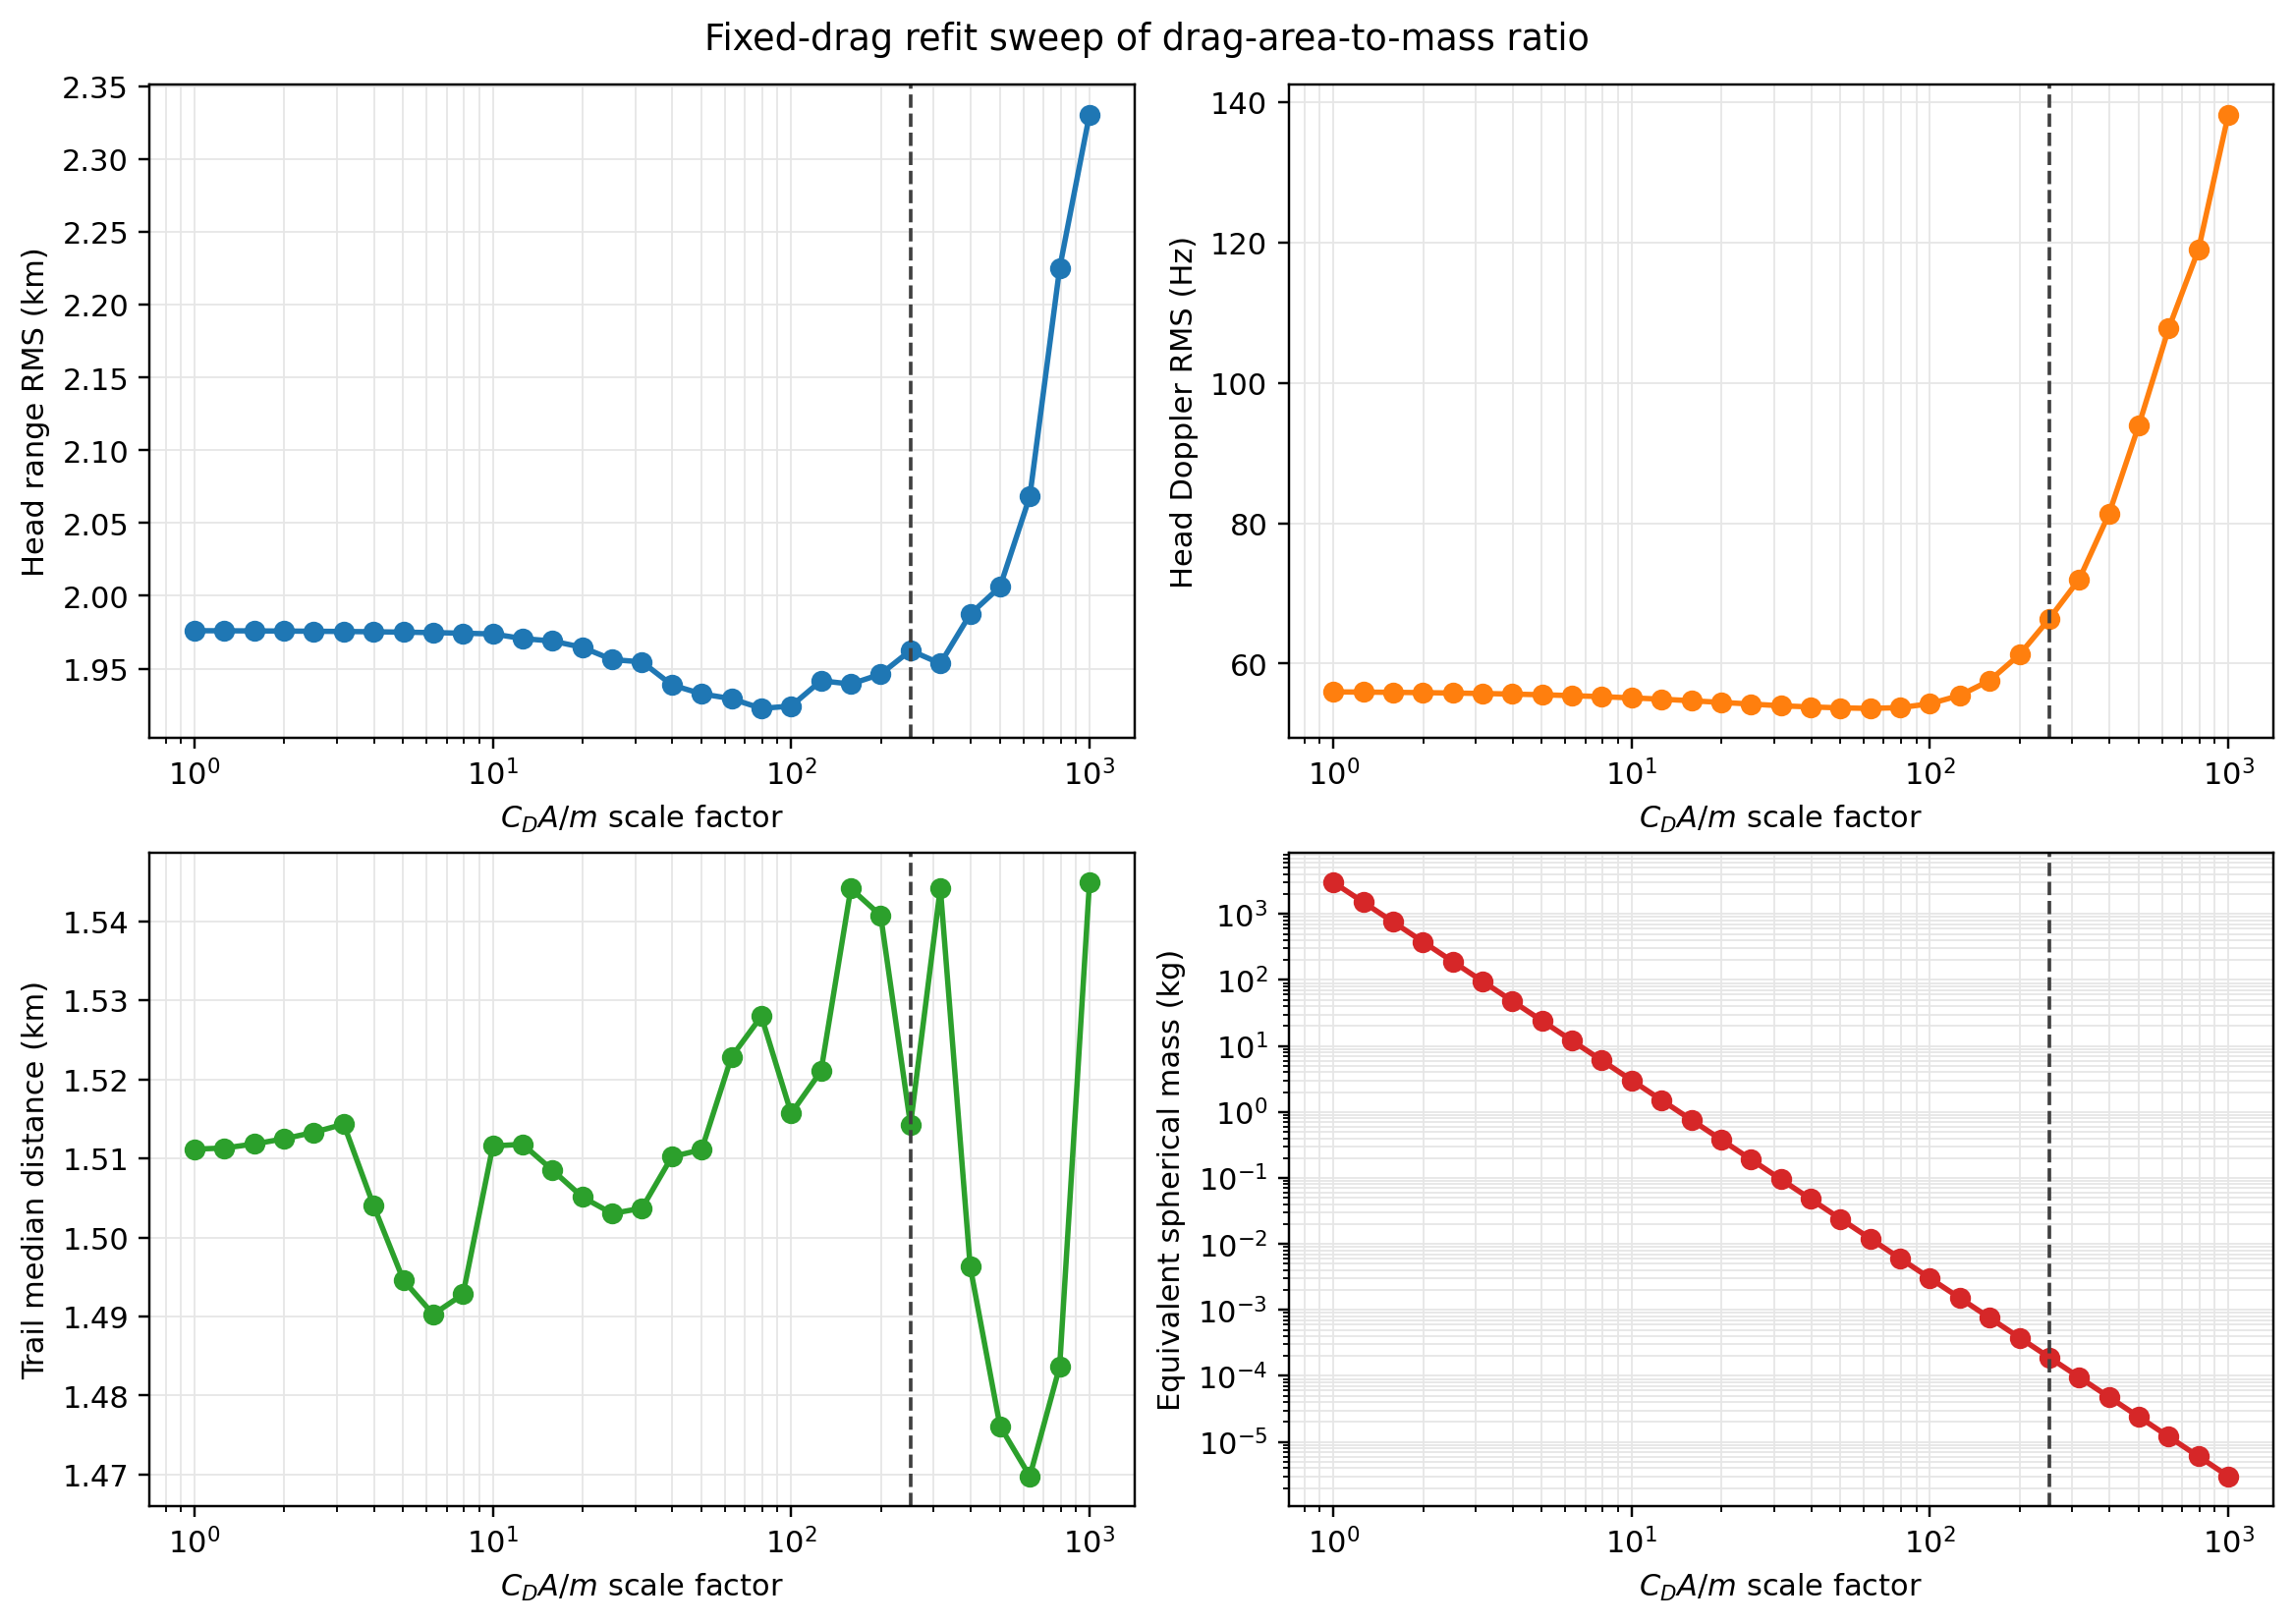
\includegraphics[width=\linewidth]{figures/ballistic_coefficient_sweep.png}
\caption{Residual growth after refitting the six initial-state components at each fixed $C_D A/m$.  The dashed vertical line marks the simple RMS-growth threshold used in this note.}
\end{figure}

\begin{table}[ht]
\centering
\caption{Residuals for fixed-$C_D A/m$ refits in the ballistic-coefficient sweep.}
\begin{tabular}{rrrrrrrrrr}
\toprule
Scale & $C_D A/m$ & Mass & Diameter & Range RMS & Doppler RMS & Trail median & $\chi^2_\nu$ & $|\Delta r_0|$ & $|\Delta v_0|$ \\
 & (m$^2$ kg$^{-1}$) & (kg) & (m) & (km) & (Hz) & (km) & & (km) & (m s$^{-1}$) \\
\midrule
1 & 4.021e-04 & 3e+03 & 1.243 & 1.98 & 56 & 1.51 & 0.075 & 1.17 & 336.2 \\
1.26 & 5.062e-04 & 1.5e+03 & 0.988 & 1.98 & 56 & 1.51 & 0.075 & 1.17 & 336.2 \\
1.58 & 6.373e-04 & 7.6e+02 & 0.785 & 1.98 & 56 & 1.51 & 0.075 & 1.17 & 336.2 \\
2 & 8.023e-04 & 3.8e+02 & 0.623 & 1.98 & 56 & 1.51 & 0.075 & 1.17 & 336.2 \\
2.51 & 1.010e-03 & 1.9e+02 & 0.495 & 1.98 & 56 & 1.51 & 0.075 & 1.17 & 336.2 \\
3.16 & 1.272e-03 & 95 & 0.393 & 1.98 & 56 & 1.51 & 0.075 & 1.17 & 336.2 \\
3.98 & 1.601e-03 & 48 & 0.312 & 1.98 & 56 & 1.50 & 0.075 & 1.17 & 336.2 \\
5.01 & 2.015e-03 & 24 & 0.248 & 1.98 & 56 & 1.49 & 0.075 & 1.17 & 336.2 \\
6.31 & 2.537e-03 & 12 & 0.197 & 1.97 & 55 & 1.49 & 0.075 & 1.17 & 336.2 \\
7.94 & 3.194e-03 & 6 & 0.157 & 1.97 & 55 & 1.49 & 0.075 & 1.17 & 336.2 \\
10 & 4.021e-03 & 3 & 0.124 & 1.97 & 55 & 1.51 & 0.075 & 1.17 & 336.2 \\
12.6 & 5.062e-03 & 1.5 & 0.099 & 1.97 & 55 & 1.51 & 0.075 & 1.17 & 336.5 \\
15.8 & 6.373e-03 & 0.76 & 0.078 & 1.97 & 55 & 1.51 & 0.075 & 1.17 & 336.7 \\
20 & 8.023e-03 & 0.38 & 0.062 & 1.96 & 54 & 1.51 & 0.075 & 1.17 & 337.2 \\
25.1 & 1.010e-02 & 0.19 & 0.050 & 1.96 & 54 & 1.50 & 0.075 & 1.18 & 338.8 \\
31.6 & 1.272e-02 & 0.095 & 0.039 & 1.95 & 54 & 1.50 & 0.076 & 1.18 & 338.8 \\
39.8 & 1.601e-02 & 0.048 & 0.031 & 1.94 & 54 & 1.51 & 0.076 & 1.21 & 345.2 \\
50.1 & 2.015e-02 & 0.024 & 0.025 & 1.93 & 54 & 1.51 & 0.077 & 1.25 & 353.9 \\
63.1 & 2.537e-02 & 0.012 & 0.020 & 1.93 & 54 & 1.52 & 0.078 & 1.25 & 353.9 \\
79.4 & 3.194e-02 & 0.006 & 0.016 & 1.92 & 54 & 1.53 & 0.080 & 1.31 & 366.8 \\
100 & 4.021e-02 & 0.003 & 0.012 & 1.92 & 54 & 1.52 & 0.083 & 1.38 & 382.3 \\
126 & 5.062e-02 & 0.0015 & 0.010 & 1.94 & 55 & 1.52 & 0.087 & 1.61 & 444.7 \\
158 & 6.373e-02 & 0.00076 & 0.008 & 1.94 & 58 & 1.54 & 0.094 & 1.71 & 464.2 \\
200 & 8.023e-02 & 0.00038 & 0.006 & 1.95 & 61 & 1.54 & 0.102 & 1.98 & 526.6 \\
251 & 1.010e-01 & 0.00019 & 0.005 & 1.96 & 66 & 1.51 & 0.113 & 2.23 & 544.5 \\
316 & 1.272e-01 & 9.5e-05 & 0.004 & 1.95 & 72 & 1.54 & 0.127 & 3.04 & 801.7 \\
398 & 1.601e-01 & 4.8e-05 & 0.003 & 1.99 & 81 & 1.50 & 0.143 & 3.25 & 809.4 \\
501 & 2.015e-01 & 2.4e-05 & 0.002 & 2.01 & 94 & 1.48 & 0.163 & 3.57 & 875.8 \\
631 & 2.537e-01 & 1.2e-05 & 0.002 & 2.07 & 108 & 1.47 & 0.188 & 4.41 & 1045.9 \\
794 & 3.194e-01 & 6e-06 & 0.002 & 2.23 & 119 & 1.48 & 0.214 & 4.52 & 992.8 \\
1e+03 & 4.021e-01 & 3e-06 & 0.001 & 2.33 & 138 & 1.54 & 0.246 & 5.06 & 1113.9 \\
\bottomrule
\end{tabular}

\end{table}
\end{document}
